\documentclass[atmp]{ipart_v1}

\Vol{19}
\Issue{3}
\Year{2025}
\firstpage{701}

\usepackage{t1enc}
\usepackage[latin1]{inputenc}
\usepackage[english]{babel}
\usepackage{booktabs}

\usepackage[skip=10pt]{caption} % Adjust the skip value as needed


\usepackage{amsthm}
\usepackage{yfonts}
\let\ltxcup\cup
\usepackage{bbm}
\usepackage{bm}
\usepackage{mathrsfs}
\usepackage{graphicx} 
\usepackage{algorithm}
\usepackage{algorithmic}


\usepackage[backend=biber]{biblatex}
%\bibliographystyle{plain} % We choose the "plain" reference style
\bibliography{refs} % Entries are in the refs.bib file


\newcommand{\comment}[1]{ \ding{118} \ding{118} \ding{118} #1  \ding{118} \ding{118} \ding{118}}
\newcommand{\bra}[1]{\langle #1|}
\newcommand{\ket}[1]{| #1\rangle}
\newcommand{\braket}[2]{\langle #1|#2\rangle}
\newcommand{\be}[0]{\begin{equation}}
\newcommand{\ee}[0]{\end{equation}}


\numberwithin{equation}{section}

\theoremstyle{plain}% default
\newtheorem{theorem}{Theorem}[section]
\newtheorem{lemma}[theorem]{Lemma}
\newtheorem{proposition}[theorem]{Proposition}


\begin{document}


\title[CayleyPY RL]{CayleyPy RL: Pathfinding and Reinforcement Learning on Cayley Graphs}

%\author[Alexander Chervov, Alexey Romanov, ... ]{Alexander Chervov, Alexander Soibelman, Alexey Romanov,  ... }

\author[A.Chervov,A.Soibelman,... ]{A.Chervov, 
A.Soibelman, S.Lytkin, S.Fironov, A.Lukyanenko, A.Dolgorukova, A.Ogurtsov,
F.Petrov, S.Krymskii, M.Evseev, L.Grunvald, D.Gorodkov, G.Antiufeev, G.Verbii, 
V.Zamkovoy, L.Cheldieva, I.Koltsov, A. Sychev, M.Obozov, 
A.Eliseev, S.Nikolenko, N.Narynbaev, R.Turtayev,
N. Rokotyan, S.Kovalev,
A.Rozanov, V.Nelin, S.Ermilov,
I.Kiselev, L.Shishina, D.Mamayeva, A.Korolkova,
%J.Naghiyev,
K.Khoruzhii, A.Romanov }

\begin{abstract}


The paper is a second in a series to develop efficient artificial intelligence based approaches to pathfinding on extremely large graphs (e.g. $10^{70}$ nodes) with focus on Cayley graphs and mathematical applications - open source CayleyPy project. The present paper proposes novel  combination of reinforcement learning approach with more direct diffusion distance approach from the first paper.  We analyze and benchmark various choices for the key building blocks of the approach:  architectures of the neural network, generators for the random works and beam search pathfinding. We benchmark these methods against the classical computer algebra system GAP and demonstrate that they  "overcome the GAP" for the considered examples.
As a particular mathematical application we examine the Cayley graph of the symmetric group with cyclic shift and transposition  generators. We provide a strong support of the OEIS-A186783 conjecture that diameter is equal to n(n-1)/2 by machine learning as well as mathematical methods. We identify the conjecturally the longest element and generate its decomposition of the desired length. Prove diameter lower bound n(n-1)/2-n/2 and upper bound n(n-1)/2+ 3n by presenting the algorithm with given complexity. Also present several conjectures motivated by numeric experiments:   the central limit phenomena - growth approximation by Gumbel distribution, uniform distribution for the spectrum of the graph and study numerically  "sorting networks", etc. 
To stimulate the crowdsourcing activity we create challenges on the Kaggle platform and invite to improve and benchmark approaches on Cayley graph pathfinding and other tasks.

% Draft: 

% Plan: 

% 1) Overcome GAP with ML/RL on several Cayley graphs - not many 3-4 generator choices

% 2) develop/benchmark code for RL methods: DQN, PPO , .... for Cayley graphs distance estimation. Benchmarks will include compraison with GAP and with ideal algorithm 

% 3) Consider only several simple graphs $S_n$ Cayley graphs: with generators sets a) transpositions b) neigbour transpositions c) (12),long cycle d) may be - all 1-cycles = Birkgoff polytope 1-skeleton



\end{abstract}

\maketitle


\section{Introduction and summary}
\subsection{Broader context}
Deep learning has revolutionized various fields of research and was recognized with several Nobel Prizes in 2024.  
In recent years machine learning has been emerging as "a tool in theoretical science"~\cite{douglas2022machine}, leading to several noteworthy applications to mathematical problems:~\cite{lample2019deep,davies2021advancing, bao2021polytopes, 
romera2024mathematical,
coates2024machine,alfarano2024global, charton2024patternboost,shehper2024makes,swirszcz2025advancing}.
 
The paper presents advancements in applying artificial intelligence methods to the mathematical problem of Cayley graph pathfinding, which is equivalent to decomposing a group element into a product of generators. It is the second in a series devoted to the CayleyPy project to develop efficient machine learning based approaches and open source library to deal with extra large graphs
(e.g. $10^{70}$) with focus on finite Cayley graphs and mathematical applications.

From a broader perspective, pathfinding is a specific case of the planning problem, where one must determine a sequence of actions to transition between two given states. Similar challenges arise in robotics and games like chess or Go, where the objective is to plan moves that lead from the initial position to a winning position. Mathematically, such problems are modeled as pathfinding on graphs (state transition graphs), where nodes represent possible states, and edges correspond to state transitions based on actions or moves. The planning task then reduces to finding a path from a given initial node to one or more target nodes. The breakthrough works AlphaGo and AlphaZero~\cite{silver2016mastering}, \cite{silver2017mastering} by Google DeepMind have demonstrated that machine learning can significantly outperform previously known methods. They serve as both a prototype and an inspiration for many developments, including ours. In a nutshell, the method consists of two main components: a neural network trained to suggest the  moves from any given state, and a graph pathfinding algorithm that helps to find a path even when the neural network's predictions are not sufficiently precise. The core idea is similar across most approaches, but achieving optimal performance for each task requires analyzing and benchmarking various neural networks and graph pathfinding methods. One of the goals of this work is to present such an analysis for some particular Cayley graphs.

\subsection{Present paper: approach, benchmarks, mathematical theorems and conjectures}

\begin{figure}[h!]
   \centering
   \includegraphics[width=1.0\linewidth]{figs/LRX.jpg}
   \caption{LRX Cayley graph for $S_5$}\label{fig:LRX1}
\end{figure}


The paper presents both AI contributions and  mathematical results and conjectures. In the present we work with a particular Cayley graph defined by the L - left cyclic shift, R - right cyclic shift and X - eXchange of positions $0,1$, it will denited LRX following \href{https://oeis.org/A186783}{OEIS}. Its image for $S_5$ in shown on figure \ref{fig:LRX1}.

{\bf Developments of AI methodology.} We propose a modification deep Q-learning (DQN) method for the case of the graph pathfinding task which resolves  the so-called sparse reward problem of the standard DQN approach for graph pathfinding. The proposal combines DQN with the more simple diffusion distance approach from our previous paper ~\cite{chervov2025machinelearningapproachbeats}. An analysis and benchmarks of these approaches are presented, including tests of various neural network architectures such as transformers, convolutional networks, and perceptrons. It  is demonstrated that these methods allow to find paths for $S_n$ up to $n$ around 30 - for the particular class of generators (LRX) which are in the main focus of the present paper. We demonstrate that they "overcome the GAP" - outperform classical computer algebra system GAP on the same task which can work only up to $n$ around 20. 

{\bf Efficient pytorch implementation.} We pay significant attention to develop original highly optimized code, current version is specific to Cayley graphs of permutation groups (matrix groups will be supported later). We propose many technical solutions for fast parallel processing of large amounts of permutations which involves product computations, efficient hashing, extracting unique, etc. The code works for CPU and GPU with no change. 

{\bf One line of code  bringing  orders of magnitudes improvement.} We report a curious finding - a single-line modification in the code of our main graph pathfinding module (beam search), dramatically improves performance. This enhancement increases the feasible pathfinding size from symmetric groups $S_n$ with $n$ to $n$ around 100 (and apparently even more with better hardware). Unfortunately, this improvement is currently specific to the particular LRX Cayley graphs considered in this paper, but we hope it can be generalized. 
%However there is grain of salt - that modification is specific to the particular generators (LRX) considered in the present paper, while the main point of the rest of our methodology is completely zero prior knowledge and applicability to very general classes graphs for which Cayley graph are just examples. Nevertheless, it is  unexpected phenomena, we hope it can be generalized for the other Cayley graphs. 

%Goal - $S_{110}$. DeepMind's success with Go game with $10^{170}$ states - creates a challenge to achieve similar results in the other fields in particular for Cayley graphs, at the moment we are somewhat far from that, but there are plenty ideas not yet incorporated in our CayleyPy project and optimistically such a goal is achievable. 

Mathematical contributions. % of the present paper are following are devoted to conjecture above and more general understanding of the properties of that Cayley graph and its relatives.

{\bf LRX Cayley graphs. Diameter conjecture \href{https://oeis.org/A186783}{OEIS-A186783}.} In the present paper we restrict ourselves to one particular family of Cayley graphs for the symmetric groups $S_n$ - the ones generated by the two cyclic shifts (L) - left, (R) - right and transposition X=$(0,1)$ of the first two positions. Surprisingly, according to \href{https://oeis.org/A186783}{OEIS-A186783} it is an open conjecture that diameter of the Cayley graph is $n(n-1)/2$ for $S_n$. These generators and Cayley graphs will be denoted LRX as in OEIS. 
%Following  \href{https://oeis.org/A186783}{OEIS-A186783} we will call them LRX generators. The fact that these three permutations generate the symmetric group is rather well-known and easy (just express neighbor transpositions  $(k,k+1)$ by shift, X, shift-back and use standard fact that neighbor transpositions generate $S_n$). %LRX are used as default generators in computer algebra system GAP/SAGE.  
 % Moreover many natural questions seems to be answered - for example is there an optimal algorithm with polynomial complexity to decompose element into LRX generators, and much more. We will use that family of Cayley graphs to benchmark various approaches  as well as we will present mathematical results and conjectures. 



{\bf The longest element.} 
By implementing an efficient brute-force breadth-first search algorithm, we traverse the full LRX graphs for $n\le 14$, confirming that the longest element has a length of $n(n-1)/2$, as predicted.  Moreover, we observe that this element is always unique and follows a clear pattern - it is a product of transpositions:  $(0,1)(n-1,2)(n-2,3)(n-3,4)...$,  so we expect this  for all $n$.  
 
{\bf AI and crowd-sourcing to support the conjecture.} For that particular element we launch various versions of our pipelines and we can never find the decomposition shorter than $n(n-1)/2$. We organize a \href{https://www.kaggle.com/competitions/lrx-oeis-a-186783-brainstorm-math-conjecture/overview}{challenge} on a Kaggle platform giving that particular element for $n=2...200$ and asking to decompose it with as short length as possible - again no one found decomposition shorter than $n(n-1)/2$. Thus confirming the expectation.
%Giving more computational support for our conjecture - that the length of that element is $n(n-1)/2$. 

{\bf Rigorous lower and upper bounds.} We prove lower bound $n(n-1)/2 - n/2$  by a combinatorial argument (improving $n(n-1)/3$~\cite{babai1989small}); afterwards prove the diameter  upper bound   $n(n-1)/2 +3n$ by the algorithm  with such complexity (improving $3/2n^2$ ~\cite{kuppili2020upper}). %To the best of our knowledge these are the best estimates and algorithm. 
We also develop another algorithm which empirically shows better complexity:  $n(n-1)/2 + 1/2n$, but lacks the rigorous proof for such an estimate.  
Finally we present explicit decomposition  for the conjecturally longest element of the desired  length $n(n-1)/2$. 

{\bf Central limit phenomena for growth - Gumbel distribution.} 
Computations suggest the following conjecture: for large 
$n$, the growth function of LRX graphs follows an asymmetric Gumbel distribution. This is in the vein of field-shaping works by P. Diaconis et. al.~\cite{diaconis1977spearman, diaconis1988metrics,chatterjee2017central}, who demonstrated that the growth of the neighbor transposition graph and many related statistics asymptotically follow the Gaussian normal distribution.

We study numerically the spectrum of LRX graph and observe surprisingly uniform distribution of eigenvalues, we also analyze statistics of the paths from the longest element to the identity ("sorting networks") we observe numerically that pattern differs from the famous "sine curves" for Cayley graph of neighbor transpositions~\cite{angel2007random}; 
numerical analysis of random walks shows consistency with results of Diaconis~\cite{diaconis1993comparison} on mixing time for LRX Cayley graph. 

We also present similar analysis for the Schreir coset graph for the action of the LRX generators on binary strings consisting of $n/2$ zeros and ones (for even $n$). %(Might be thought as an analogue of Grassmanian $Gr(n,2n)$ over the field with one element.)

To conclude our analysis demonstrates that computational experiments in particular with AI component can be quite useful for advancing mathematical research on Cayley graphs. And AI methods significantly outperform classical methods of computer algebra systems like GAP, performing well for  $S_n$ with $n$ around 30, and with small addition of prior knowledge up 90, while classical methods only up 20. 


% \begin{itemize}
% \item We reproduce and extent OEIS analysis confirming the conjecture by brute force computations till $n\le 14$ (extending $n \le 13$ in OEIS) and computing full growth polynomials. 
% \item We observe that there is a unique longest element which can described as a product of transpositions $(0,1)(n-1,2)(n-2,3)(n-3,4)...$ for all $n\le 14$ and conjecture it is true for all $n$.
% \item 
% \end{itemize}

%In the present paper we re


\subsection{Finite Cayley graphs: pathfinding techniques, results and open problems}

Let us briefly summarize existing techniques for Cayley graphs pathfinding, and remind more general context on Cayley graphs research.


{\bf Optimal pathfinding is typically NP-hard.} Finding the shortest paths on generic finite Cayley graphs is an NP-hard problem~\cite{even1981minimum} (even P-space complete \cite{jerrum1985complexity}). As is the case for many specific group families, such as NxNxN Rubik's Cube groups~\cite{demaine2017solving} and others~\cite{bulteau2015pancake, wilson2024cayley}.
For particular groups it is hard to develop practical optimal algorithm e.g. standard 3x3x3 Rubik's cube the first optimal algorithm has been proposed only 1997~\cite{korf1997finding}. It required 192 Gigabytes of precomputed data and 12-24 hours to solve single cube (methods were later improved\cite{Reid1997Optimal,HKociemba2021,Rokicki2014Diameter,Skalskivcube} to several cubes per second). To develop practical optimal solver for 4x4x4 Rubik's cube - is a challenge. 

{\bf Non-optimal pathfinding: Schreier-Sims algorithm, GAP implementation, non-effectivity for large groups.} 
The Schreier-Sims algorithm~\cite{sims1970computational},\cite{knuth1991efficient} (or its randomized versions) is the method typically used for decomposing group element into product of generators for permutation groups. It is implemented in GAP computer algebra system. However its outputs "are usually exponentially long"~\cite{fiat1989planning} and that forbids practical computations for large groups (typically the sizes beyond $10^{30}-10^{40}$ are out of reach - examples and analysis is given below). 

{\bf Non-optimal pathfinding: "small support" Kaggle Santa 2023 methods (generality issue).} The methods which can deal with extremely large groups (e.g. size $>10^{1000}$ like 33x33x33 Rubik's cube) were demonstrated by top participants of the recent challenge organized on the Kaggle platform - \href{https://www.kaggle.com/competitions/santa-2023}{Santa 2023}. However the generality of that approach is unclear.%What is not clear whether  such methods be applied only to some specific choices of generators or can be extended to any choices. 
That is contrast to AI methodology which is from the beginning is  general not even restricted to Cayley graphs. The idea of "Santa methods" is quite noteworthy:  one should first find "small support elements" achievable from original generators and take them as new generators, then one simply runs beam search with Hamming distance heuristics to find path. Method becomes effective since for small support generators Hamming distance and true graph distance are  quite related by obvious reason. "Small support" are those permutations which change only small number of positions. They are well-known for  Rubik's cube solvers - "commutator" or "Pif-Paf" moves~\cite{mulholland2016permutation}, \href{https://math.stackexchange.com/q/4962862/21498}{M.Brandenburg post}. In mathematics small support elements play an important role in deep works by Babai, Seress, Helfgott, et.al.~\cite{babai1988diameter, babai2004diameter, bamberg2014bounds, helfgott2014diameter, helfgott2019growth} (slides: \href{https://www.math.auckland.ac.nz/~conder/SODO-2012/Seress-SODO2012.pdf}{A.Seress},\href{https://simons.berkeley.edu/sites/default/files/docs/6206/symtalk.pdf}{H.Helfgott} ), however it is 
unclear whether one can effectively find small support elements from given generators, thus making unclear the generality of "small support methods".

{\bf Non-optimal pathfinding: algorithms for specific families of generators.} 
For some particular choices of generators there are algorithmic solvers which can effectively find non-optimal solution. It seems unlikely that one can produce similar algorithms for any generators. The prototypical example is bubble sort algorithm, which solves the problem for the neighbor transpositions generators of $S_n$. Algorithmic solvers exist for Rubik's cube of arbitrary sizes and for other puzzles related groups. The other families of generators  and algorithms are important in bioinformatics for estimation of the evolutionary distance. These generators are related to flips of subsequences - see e.g.~\cite{Pevzner1995human2mice, Pevzner1999cabbage2turnip, wilson2024cayley, bulteau2019parameterized}. Related example is \href{https://en.wikipedia.org/wiki/Pancake_sorting}{pancake sorting} (or prefix sorting) problem with the first algorithm proposed by Bill Gates et.al. \cite{gates1979bounds}.

{\bf AI-methods for pathfinding.} 
To the best of our knowledge there is no systematic effort for Cayley graph pathfinding  with AI methods except our CayleyPy project. However for some particular cases for example Rubik's cube there exists a number of approaches, e.g. based on genetic algorithms:~\cite{swita2023solving}.%, which can be modified for the general case. 
The most notable are: DeepCube~\cite{mcaleer2019solving, agostinelli2019solving, khandelwal2024towards,agostinelli2024q} - the first AI based successful solver for 3x3x3 cube (\href{https://deepcube.igb.uci.edu/}{website}), the second one: EfficientCube~\cite{takano2023selfsupervision}, some other:~\cite{brunetto2017deep,johnson2021solving,amrutha2022deep,noever2022puzzle,chasmai2022cubetr,bedaywi2023solving,pan2021fourier} which not achieve complete solution. Noteworthy idea~\cite{pan2021fourier} is to combine neural networks with representations theory of the symmetric group ---  neural net  predicts the coefficients of the non-abelian Fourier transform for the distance function. The rationale is: observed sparsity (bandlimitedness) of Fourier transform of the common distance functions on $S_n$ ~\cite{swan2017harmonic}. The recent seminal achievement from S.Gukov's team: ~\cite{shehper2024makes} creates effective AI based pathfiding approach for infinite group of Andrews-Curtis moves and resolves the  Akbulut-Kirby conjecture remained opened for 39 years. AI-methods are also used for pathfinding in the context of planning movements in obstacle-rich environments and road networks it is related field, but with different focus \cite{pandy2022learning, kirilenko2023transpath} 

{\bf Cayley graphs: applications, diameters, random walks, open conjectures.}
Let us give a more general context on Cayley graph research.
Cayley graphs are fundamental in group theory~\cite{gromov1993geometric},\cite{tao2015expansion}, and have various applications: bioinformatics
~\cite{Pevzner1995human2mice, Pevzner1999cabbage2turnip, wilson2024cayley, bulteau2019parameterized}; processors interconnection networks~\cite{akers1989group, cooperman1991applications,heydemann1997cayley};in coding theory coding theory and cryptography~\cite{hoory2006expander,zemor1994hash,petit2013rubik}; in quantum computing~\cite{ruiz2024quantum,sarkar2024quantum,dinur2023good, acevedo2006exploring,gromada2022some}, etc.

%{\bf Cayley graphs: applications, diameters, random walks, open conjectures.}

Two focuses of pure mathematical research on finite Cayley graphs are related to diameters estimation and the behavior of random walks. In the case of the symmetric group $S_n$ there are two open conjectures which are easy to formulate, but somewhat representative for the field.  

{\bf Babai-like conjecture:} diameter of  $S_n$ is not more than $O(n^{2})$ - for any choices of generators (see e.g. H.Helfgott's surveys: ~\cite{helfgott2014diameter},\cite{helfgott2019growth},\cite{helfgott2015random} ; 

{\bf Diaconis ~\cite{diaconis2013some} conjecture:}  the mixing time for random walks is not more than $O(n^{3}log(n))$ (again for any choices of generators). 

The first one can be thought as a particular case of the Babai conjecture~\cite{babai1992diameter},\cite{tao2015expansion} which predicts that diameter of simple groups is not  large as one may expect: $O(log^c|G|)$ for some absolute $c$ --- in contrast to abelian groups where it can be $O(|G|)$.  Thus conjecture represents an intriguing connection between algebraic properties of a group (which does not depend on the choice of generators) - being simple  and the  property of Cayley graphs - having short diameter (which is generator dependent property). 



%Cayley graphs are fundamental for geometric group theory~\cite{gromov1993geometric} which mainly focuses on infinite groups, where  some properties of graphs (like growth) do not actually depend on choices of generators and represents internal properties of groups.

%Cayley graphs of finite groups is also active field of research in pure mathematics~\cite{tao2015expansion}, and have various applications:in  bioinformatics  for estimating evolutionary distance~\cite{Pevzner1995human2mice},\cite{Pevzner1999cabbage2turnip},\cite{wilson2024cayley},\cite{bulteau2019parameterized}; processors interconnection networks~\cite{akers1989group},\cite{cooperman1991applications}, \cite{heydemann1997cayley};in coding theory for construction of expander graphs and related codes~\cite{hoory2006expander};in cryptography to construct specific hash functions~\cite{zemor1994hash},\cite{petit2013rubik};in machine learning~\cite{wilson2024cayley}; in quantum computing~\cite{ruiz2024quantum},~\cite{sarkar2024quantum},~\cite{dinur2023good},~\cite{acevedo2006exploring},~\cite{gromada2022some}.
 

Estimating diameters of Cayley graphs is a hard problem. One of it applications is latency estimation for processor interconnection problem~\cite{akers1989group},\cite{cooperman1991applications}, \cite{heydemann1997cayley} - since diameter corresponds to maximal latency. 
It is also question of interest for community of puzzles enthusiasts - like Rubik's cube. Diameter is also called a "God's number" - the number of moves the worst configuration can be solved by the best algorithm. It is widely unknown for most of the puzzles, its determination for the Rubik's cube 3x3x3 for the standard choices of generators required significant efforts and computational resources~\cite{Rokicki2014Diameter}.  It is not known precisely for higher cubes, neither for 3x3x3 Rubik's with \href{https://www.speedsolving.com/wiki/index.php?title=Metric#STM}{STM, ATM} metrics.% cube with a little modified definitions of generators.  
A precise conjectures on 4x4x4 and 5x5x5 Rubik's cube diameters appeared recently~\cite{hirata2024probabilistic}, collections of conjectures and estimates for many puzzles can be found on \href{https://www.speedsolving.com/wiki/index.php?title=God%27s_Algorithm#Table_of_God.27s_Numbers}{speedsolving website}. 

As we will discuss below novel AI methods might provide insights via computational experiments to such kind of questions.

%\subsection{Finite Cayley pathfiding: approaches, algorithms, NP-hardness results}
%Let us discuss state of the art and "competitor analysis" for the pathfinding problem. 

\section{Reinforcement learning (RL) and graphs pathfiding}
\subsection{Reminders: RL, sparse reward problem, Bellman equation for graph distances,  Q-algorithm, pathfinding}

{\bf RL in brief.}
Reinforcement learning is an important direction 
in AI which is different from supervised and unsupervised learning in the following respects: it aims to optimize {\bf cummulative} reward and it requires from the agent to in a sense to "{\bf create train set by himself}", agent should choose best strategies to "explore the space" and select training examples by himself, in contrast to the supervised learning where the training set is given a priory. 

{\bf RL "equivalence" to graph pathfinding. }
The setup of reinforcement learning is very similar to the setup of graph pathfinding: states - are nodes of the graph, actions corresponds to edges/transitions to neighbor states by these edges, rewards corresponds to weights on the edges. The cumulative reward corresponds to  length of paths (with respect to edges weights). Typically in graph theory shortest paths are of interest - that means "reward" is minimized, not maximized as in RL, so it is better to use term not the "reward", but "penalty". 

{\bf Unweighted graphs and sparse reward problem.}
Sparse reward problem is the famous problem in RL and it exactly appears in Cayley graphs pathfinding and more generally for pathfinding on any unweighted graph, thus making standard RL approaches poorly performing.
The sparse reward problem is a situation where the reward is given very rarely and thus  it is difficult to generate the data for training. That situation exactly happens for graph pathfinding on large graphs - where one needs to find a path to say a one selected node out of trillions of other nodes. Reward is given only by finding the desired node - but it is practically impossible to find it with a "cold start" by random. Pay attention that condition on all weights equal to one - play a role - if weights would be different - one may hope strategy to choose the  step with best local reward is reasonable, however when all weights are exactly the same, there is no local preference to make a right move. 
There are several strategies to resolve that issue and below we propose a new one below. 

{\bf Bellman value equation  is equation for distance functions.}
The value function (or "position estimation") in RL exactly corresponds to the distance functions on graphs. 
To make that analogy more precise: consider an unweighted  graph $G$ (all edges weights are equal to 1), choose some node $e$ (e.g. identity of a group in Cayley graph), consider a function $d(g)$ - the distance of the shortest path from $g$ to $e$ (it is "\href{https://en.wikipedia.org/wiki/Word_metric}{word metric}" in group theory). Then there is an simple relation:

\begin{align} 
%$$ 
\label{bel_eq}
d(g) & = 1 + \min_{n:~neigbours~of~g} d(n)  \text{~~~Bellman equation}\\
%$$
d(e) & = 0 \text{~~~boundary condition}
\end{align} 

This relation is simple, but it is fundamental - it is a particular case of the Bellman's equation. The properties can be summarized in the following simple proposition, which is easy to see inductively considering neghbor nodes to $e$, then neighbors of neighbors and so on.

\begin{proposition}
    For any finite connected graph $G$ the only solution to the pair of equations above are given by the  distance function (length of the shortest path) to the node $e$. Moreover the only solutions to the Bellman's equation (without boundary condition) correspond to distance to some sets of nodes in $G$ (up to adding a constant). That set can be recovered as minimums of $d(g)$. 
\end{proposition}

{\bf Sense of Bellman equation - local condition for globally (cumulatively) defined object.}
The Bellman equation is equation for the length of the shortest path - that is globally/cumulatively defined object, but the condition itself is local - only at the neighbor of each point.  

{\bf Idea of Q-learning and deep Q-learning algorithms for value/distance function.}
These algorithms provide a way to compute solutions of the Bellman equation, which means to find the distance functions on graphs.  One starts with some  initialization for $d(g)$, then just  the new approximation $d_k(g) = 1+\min_{n:~neigbours~of~g} d_{k-1}(n), d_{k}(e) =0$ by applying the right hand side of the equations \ref{bel_eq}. There are theoretical guarantees that such a process will converge to the solution of the Bellman equation (and boundary condition). 

{\bf Idea of deep Q-learning algorithm.}
The deep Q-learning is used in the situations where the graph is large (can be of google size). 
One assumes that for each node of graph there is a feature vector attached. 
One considers a neural network which takes a feature vector as an input and should output the approximate solution for Bellman equations.
The training process is organized as follows.
Each epoch one selects some subset of nodes and from current neural network $d(g)$  computes the right hand side of the equations \ref{bel_eq}
$t(g) = 1+\min_{n:~neigbours~of~g} d(n), t(e) =0$, denoting $t(g)$ as a result of that computation. 
Afterwards one runs gradient descent to minimize the error between $d(g)$ and $t(g)$. If the error would be zero that means that $d(g)$ solves the Bellman equations. And thus in graph theory setup it produces the distance function ("word metric" in case of Cayley graphs).
Typically the choice of the training subset of nodes  is made with the help of walking over the graph combining both random steps and steps guided by the model. We will discuss that in details below.

{\bf Graph path finding.}
To find a path from a given node $g$ to the selected  $e$ one just need to run greedy search algorithm, which starting from node $g$ inspects all its neighbors and evaluates distance function for them, then chooses the the node with the minimum value of the distance function and makes a move to that node. The process is repeated untill the number the destination node is found on the steps limit is exceeded. In case the distance function is the true distance on the graph (the lenght of the shortest path) such algorithm find the shortest path and finds it in the optimal way (least possible operations). However in the case of deep Q-learning typically the predictions of the neural network are not very precise, and greedy algorithm will stuck on local minimums. To overcome that difficulty one used more advanced graph search algorithms like beam search, or A-star, etc. That is discussed below.

\subsection{Diffusion distance pathfinding - CayleyPy-1}
Let us briefly remind the alternative pathfinding approach proposed in our previous paper \cite{chervov2025machinelearningapproachbeats}. Its efficiency has been demonstrated on the Rubik's cube where it significantly outperforms all possible competitors providing shorter solutions than any existing approach for 3x3x3,4x4x4,5x5x5 cubes. And in some sense it is more simple and computationally efficient. 

The idea of the approach is to work not with the true distance on the graph, but with the diffusion distance which might be thought as a length of the random path. The diffusion distance is easy to estimate by the number of steps of random walks. Generation of random walks is much more fast than computations of the neural networks predictions, thus generation of the training data is much more efficient than in Q-learning approaches, though the training data might be of weaker quality. 
The assumption is that for each node of a graphs there is feature vector attached. For example for permutation groups it is a vector representing a permutation $(p_0,p_1,p_2,...p_{n-1}), p:i \to p_i $
We also assume that there is a selected node (e.g. identity of the group) where we need to find a path from any other node. 

Core of the approach consists of the three steps:

\begin{enumerate}
    \item {\bf Generation of training set by random walks.} 
    Generate $N$ random walks trajectories all starting from a selected node $e$ (identity of a group). Each random walk trajectory consists of up to $K_{\text{max}}$ steps, where $N$ and $K_{\text{max}}$ are integer parameters of the method. For some nodes encountered during the random walks, we store a set of pairs $(v, k)$, where $v$ represents the vector corresponding to the node and $k$ is the number of steps required to reach it via the random walk. 
    \item {\bf Generation of training set by random walks.}  The generated set of pairs $(v, k)$ serves as the training set for the neural network. Specifically, $v$ serves as the 'feature vector' (the input for the neural network), and $k$ represents the 'target' (the output that the network needs to predict). Thus, the neural network's predictions for a given node $v$ estimate the diffusion distance from $v$ to the selected destination node.
    \item {\bf Graph search guided by neural network. Beam search.} This step finds a path from a given node to the destination node. The neural network provides heuristics on where to make the next steps, while the graph pathfinding technique compensates for any possible incorrectness in the neural network predictions. The beam search pathfinding method is quite simple, but has proven to be the most effective for us and works as follows. Fix a positive integer $W$ - a parameter known as the "beam width" (or "beam size"). 
    Starting from a given node, we take all its neighboring nodes and compute the neural network predictions for all of them. We then select the $W$ nodes that are closest to the destination according to the neural network (i.e., the predictions have smaller values). For these selected $W$ nodes, we take their neighbors, drop duplicates, and again compute the neural network predictions, choosing the top $W$ nodes with the best (i.e., minimal) predictions. This process is repeated until the destination node is found (or limit of steps is exceeded).
  
\end{enumerate}

The last step is common for all methods - based on Q-learning or diffusion distance. One uses a neural network predictions as heuristic function and uses graph search algorithms to find a path. We are strongly in favor of beam search, while DeepCube team~\cite{mcaleer2019solving, agostinelli2019solving, khandelwal2024towards,agostinelli2024q} develops A-star algorithm and its modifications.

\subsection{Beam search effectivity - toy model of research community }

To some extent the success of the scheme proposed above is due to beam search (we started from modified greedy search, then Metropolis, then A-star and finally beam search was a relief). It is import to achieve as big beam sizes as possible, that it achieved by effective pytorch implementation which  is capable to support beam sizes with millions nodes and more  nodes. On the one hand beam search is probably one the most simple methods, on the other hand there is several moments which are less obvious. It deserves to comment on them. 

The first simple reason why simple reason to explain why we need beam search is problem of local minimums. The greedy search will be stucked in them, but beam search will not even notice local minimums if the beam size is larger than depth of local minimums. 
It like an elephant will not even notice small minimums of the surface, while for ant that can be insurmountable obstacle. 

The other moment about beam search that increasing beam size not only linearly increases the computations, but also linearly increases the memory consumption. It is on the one hand the main bottleneck of the method - memory - not the computational time, but on the hand it is somewhat critical for its performance to have as much beam size as possible. Moreover there is no easy way to reproduce results of beam search with beam size $B+1$ with any algorithm of with memory consumption $B$.  

To explain that point we will use the analogy with the work of research community.
Imagine two researchers working on some creative problem together (beam of size 2). The key point is the exchange of ideas --- if one researcher finds a break-through he shares with the other and they continue search from the break-through point, if that exchange would not happen the second researcher would probably be stuck in some dead-end.  So the exchange of ideas allows not to waste time on those direction which are useless. 
The mechanism above is exactly the one which explains why increasing the beam width is so effective - it is a kind of exchange of ideas, concentrating on breakthroughs, not following dead directions.  Indeed, that is essentialy what beam search is doing: we select the top nodes which were neighbors for the entire beam --- but not select several best for the first node, several for the second and so on. Thus if neighbors of one node are much closer to destination (analog of break-through) we keep these nodes in the beam and sacrifice neighbors for the less successful nodes (in the other words descendants of some nodes do not survive in the next generation).

The size of research community matters, cutting down community say twice, will not decrease the research output twice - but it will decrease it exponentially, the same for beam search - the size matters, and there is no easy way to achieve performance with beam size $B$ using smaller beam.

That logic also explains why the so-called evolutionary or nature inspired global optimization methods are sometimes successful, they provide the same mechanism, but offer better control of the diversity of beam size. Because sometimes it is important not to jump to the breakthroughs made by the others - but continue to work in your own direction, and it migth probably lead to a bigger breakthrough. The balance between "everybody jumps to new breakthrough" (like in beam search), and keeping the diversity is subtle, apperently there is "no free lunch" and different tasks require diferent balances. That is direction to be explored for Cayley graphs pathfinding. 



\subsection{Proposal -  combining diffusion distance with deep Q-learning}

{\bf Rationale. Why we need that?} The diffusion distance approach described above is quite simple and efficient however there is practical and theoretical disadvantage. The practical side consists of somewhat surprising phenomena that enlarging the training set (generating more random walks) does not always improve the quality of the model - such stagnation was  observed for Rubik's cube cases in our previous paper and it is even more prominent for LRX graphs. It is actually related to the quite clear theoretical fact: diffusion distance is not monotonically dependent on the true distance - one node can be further than another for the true distance, while oppositely ranged for the diffusion distance. (That problem is not only for random walks estimation, but for the diffusion distance itself (i.e. limit of infinite data - computed theoretically (\href{https://www.kaggle.com/code/fedmug/lrx-diffusion-distance-analysis}{analysis}) ). %Such phenomena will be discussed below in more details (see also our n with analysis). 
So diffusion distance is easy to estimate, but it is not precise. On the other hand DQN and Bellman equation allows to approximate the true distance, but for the price of more heavy computations. 
The idea of the proposal below is to combine less precise but light weight diffusion distance with more heavy and more precise Bellman equation approach. And to avoid the sparse reward problem.

Our proposal looks as follows.

{\bf Warm-up  diffusion distance training. } Use the diffusion distance approach for preliminary training the neural network. I.e. apply the steps 1,2 above: generate random walks to create training data, and train neural network to predict number of steps of random work.

{\bf Modified DQN training. }
The second phase will relies on the Bellman equation strategy with mild modifications, but on somewhat different space exploration strategy comparing to conventional DQN - borrowed from the diffusion distance approach:

Step 1. Generate $N$ non-backtracking random walks trajectories all starting from a selected node $e$ (identity of a group). Each random walk trajectory consists of up to $K_{\text{max}}$ steps, where $N$ and $K_{\text{max}}$ are integer parameters of the method. 

Step 2. For the obtained nodes compute the Bellman equation predictions
$t(g) = 1+\min_{n:~neigbours~of~g} d(n), t(e) =0$ in the standard way. 

Step 3. Clip the predictions by the number of steps of the random work since true distance is always smaller than number of steps. (Clip also predictions negative values). 

Step 4. Run gradient descent for the neural network to minimize the loss function between clipped $t(g)$ (target) and neural network predictions. 

{\bf Graph search algorithm - beam search with neural network as an heuristics. } After the neural network is trained we utilize the same approach to find a path by beam search and neural network as in our previous paper.


The advantages of the proposed method are the following: there is no sparse reward problem - since we always start from the selected state, it always allows us to clip overestimated predictions, the warm-up phase allows to avoid long initialization process until when targets obtained by Bellman equation random since network starts from random weights - in our approach targets are always meaningful - first they are steps of random walks, at the second phase neural by itself produces meaningful targets since it was preliminary trained. We also suggest to use non backtracking random walks by rather clear reason - number of steps for non-backtracking is more similar to true distance. Conceptually that is related to the well-known phenomena - "Non-backtracking random walks mix faster"\cite{alon2007non}.

{\bf Benchmarks and analysis.}
Below we present the analysis of that proposal. 
We observe  stable improvement of the method above comparing to diffusion distance approach, unfortunately the effect is not so big.  

The first experiment is concerned not large groups, where one can compute by brute force the true graph distance and compare it with the predictions of the neural network. We see that for small sizes of the group methods learn practically ideally the distance on a graph, however for large groups correlation becomes not so perfect. Additional training by DQN always improves the preliminary warm-up training by diffusion distance procedure. 


\begin{table}[h]
    \centering
    \begin{tabular}{|c|c|c|c|c|}
        \hline
        $n$  & epochs: 5+0  & epochs: 50+0   & epochs: 5+50   & epochs: 50+50  \\
        \hline
        6 &  0.955 & 0.99  & 0.99  & 0.99 \\
        8 &  0.954 & 0.969 & 0.98   & 0.982 \\
        10 & 0.883  & 0.923 & 0.939   &  0.938 \\
        \hline
    \end{tabular}
    \captionsetup{skip=10pt} 
    \caption{n - permutation length. Spearman correlation of the true distance (obtained by brute force on million states) vs predictions of the neural networks trained by different methods. Conclusion Additional training with DQN improves results. Epochs A+B denotes: A - training epochs in warm-up diffusion distance part, B - epochs in DQN part.  }
    \label{tab:example}
\end{table}

The second experiments concerns larger group $S_{28}$ with LRX generators. We train the model and search for path by the beam search. The length of the path is the measure of performance. Experiment confirms that additional training by DQN improves the results. The combinatation of the 30+200 epochs training with 30-warmup and   200 - second stage (DQN) - is one the best which we observed for that case. Average length is 402, best is 382 which is not far from the expected ideal length 378. (In all experiments we searched path from the same element - conjecturally the longest element for LRX generators). For each experiment models for retrained from scratch, thus due to random nature of the random walks models are significantly different. 
\begin{table}[h]
    \centering
    \begin{tabular}{|c|c|c|c|c|c|}
        \hline
        Experiment  & epochs:  & epochs:   & epochs: & epochs:    \\
                    &  30+200  &  30+0   & 100+0 &  0+230   \\
        \hline
        1 &  490 & None  & 446  &  None \\% AC
        2 &  396 & 658   & 516  &  None \\% AC
        3 &  382 & None  & None  & None  \\% AC
        4 &  408 & 650   & 436  &  None \\ % AC
        5 &  428 & 706   & 1046  & None  \\ % Firnov
        6 &  396 & None  & None  & 508  \\ % Fironov
        7 &  426 & 890   & 614  &  None \\ % Fironov
        8 &  None& 598   & None &  None \\ %Rustem
        9 &  392 & 464   & 524  &  None  \\ % Shishina
        10 & None& 626   & 452  &  434 \\ %Liuda 
        Median & 402& 650   & 516 &   \\
        \hline
    \end{tabular}
    \captionsetup{skip=10pt} 
    \caption{Lengths of solutions obtained by different approaches. 
    $S_{28}$ LRX generators. 10 experiments to decompose the "longest" element with expected ideal length 378. Conclusion: additional training by DQN improves the results - both in length and probability to find a path. Pure DQN training is not performing well. }
    \label{tab:example}
\end{table}

The analysis can be found in \href{https://www.kaggle.com/code/alexandervc/lrx-cayleypy-rl-mdqn}{notebook}.  

\section{Benchmarks}

Goal - $S_{110}$. DeepMind's success with Go game with $10^{170}$ states - creates a challenge to achieve similar results in the other fields in particular for Cayley graphs, at the moment we are somewhat far from that, but there are plenty ideas not yet incorporated in our CayleyPy project and optimistically such a goal is achievable in near horizons. Moreover in the present study we achieve pathfinding for such scale groups, but unfortunately not by fully zero prior knowledge. Our zero prior knowledge approaches achieves pathfiding for  LRX generators of $S_{n}$ a bit above $30$, but at the moment  $40$ is a not achieved despite  bunch of neural networks we tried. What is surprising that almost all approaches we tried stuck slightly above $n=30$ - all in the same region, with small variations. It is significantly better than results of computer algebra system GAP which achieves only about $n=20$, which much more lengths and timings. 
%But somewhat far from the desirable goal

\subsection{One line of code to get orders of magnitude improvement from: $S_{30+}$ to $S_{100+}$. }

\texttt{if action == 'X' and current-state[0] < current-state[1]: continue }
The condition used in the beam search part. Its logic is rather clear - if the positions 0 and 1 are already sorted - it is logical not to swap them i.e. not to apply $X$ generator. 

Surprisingly such a simple conditions is a game changer. Inserting it and using it with exactly the same pipelines which performed for around $n=30+$ we  are able to find paths for $n=100$ and (apparently more - just stopped by 16G RAM limit). So the size of graphs changes from $10^30+$ to $10^150+$.  It works the same for all models: perceptrons, gradient boostings, convolutional neural networks.  

The challenge is how to avoid such prior knowledge method and extend it to other generators.

It should also be noted that this condition prevents to find optimal paths. And for small sizes of $n$ it typically leads to a bit longer paths, but for high values of $n$ it is a relief.

The lengths of the paths found by this method are for example the following:

\begin{table}[h]
    \centering
    \begin{tabular}{|c|c|c|c|c|c|}
        \hline
        $S_n$  & 100 & 90   & 80  & 70 & 60  \\
        \hline
        length        & 16632 & 33459  & 7510  & 8115 & 3650 \\
        \hline
        ideal length &  4950   & 4005  & 3160  & 2415 & 1770 \\
        \hline
        Time         &  8h 43m & 3h 57m   & 1h 5m  & 52m & 3h  \\
        \hline
        Nb version   &   255   &  242     & 241    & 233  & - \\
        \hline
    \end{tabular}
    \captionsetup{skip=10pt} 
    \caption{n - permutation length. Lengths of solutions for different $n$.   }
    \label{tab:example}
\end{table}

Computation for $n=100$ took 8h 43m 53s GPU P100. Beam width $ {2}^{20}$, 30 epochs of training. ( \href{https://www.kaggle.com/code/alexandervc/lrx-cayleypy-rl-mdqn?scriptVersionId=223954525}{Notebook version 255}), for other cases we used beam size not more than $ {2}^{18}$, that is why for $n=90$ length is much bigger. The data for $n=60$ is obtained by the gradient boosting model, with slightly better lengths, but more timing.

\subsection{"Overcome the GAP" with zero prior knowledge AI. }

We use LRX Cayley graph of $S_n$ and its conjecturally longest element of expected length $n(n-1)/2$ as a benchmark. Below we demonstrate that AI methods significantly outperform classical methods of computer algebra system GAP. 

\begin{table}[h]
    \centering
    \begin{tabular}{|c|c|c|c|c|c|}
        \hline
        $n$  &  GAP    & Ideal            &   AI      \\
             &  Length & Length n(n-1)/2  & Length    \\
        \hline
        9    &  41     & 36               &  36   \\
        \hline
        10   &    51   & 45               &  45       \\
        \hline
        11   &     65      & 55             &  55     \\
        \hline
        12   &    78       &  66          & 66     \\
        \hline        
        13   &    99       &  78           &   78       \\
        \hline        
        14   &   111       &  91           &   91     \\
        \hline        
        15     &   268      &  105         &  105    \\
        \hline        
        16     &    2454    &  120         &  120     \\
        \hline        
        17   &     380     &  136         & 136    \\
        \hline        
        18   &     20441   &   153        & 153    \\
        \hline        
        19   &      3187      & 171        & 171    \\
        \hline      
        20   &     217944    & 190        & 190      \\
        \hline 
        21   &   -           & 210     & 210        \\
        \hline           
    \end{tabular}
    \captionsetup{skip=10pt} 
    \caption{n - permutation length. Comparison of GAP vs AI methods. On the conjecturally longest element of LRX Cayley graph. Its expexted length is $n(n-1)/2$.  }
    \label{tab:example}
\end{table}
For $n=20$ GAP timing is 41min 18s on while AI methods can find results much faster.
For example, simple neural network: \href{https://www.kaggle.com/code/alexandervc/lrx-cayleypy-rl-mdqn?scriptVersionId=224270083}{notebook version 423}: 3m 48s GPU P100.

\begin{table}[h]
    \centering
    \begin{tabular}{|c|c|c|c|c|c|}
        \hline
        $n$  &   Ideal            &   AI      \\
             &   Length n(n-1)/2  & Length    \\
        \hline
        22    &       231           & 231   \\
        \hline
        23    &       253           & 253   \\
        \hline
        24    &      276            & 276   \\
        \hline
        25    &    300              & 300   \\
        \hline
        26    &     325             & 325   \\
        \hline
        27    &     351             & 351   \\
        \hline
        28    &     378             & 378   \\
        \hline
        29    &   406               & 408   \\
        \hline
        30    &     435             & 437   \\
        \hline
        31    &    465              & 478   \\
        \hline
        32    &    496              & 728   \\
        \hline
        33    &    528              & 642   \\
        \hline           
    \end{tabular}
    \captionsetup{skip=10pt} 
    \caption{n - permutation length. Comparison of GAP vs AI methods.   }
    \label{tab:example_nn}
\end{table}

Here we collect results of several type of models gradient boostings and neural networks, all of them quite stably and perfectly solve cases with  $n\le 30$, but beyond requires efforts for all models.%, and in several steps in $n$ they loose ability to find a path. 
It is surprising that all types of model have the problem at the same range $n$ and that length is not becoming gradually longer and longer, but  it  stays almost perfect, and then  quite sharply pipeline loses ability to find a path at all. For some cases  we use several reruns - if the path not found via single run, it sometimes be found by multiple relaunches of the pipeline. 
For example $n=32$ has been solved with our modified DQN strategy with 30 warmup epochs and 1000 DQN epochs (\href{https://www.kaggle.com/code/rustemturtayev/lrx-cayleypy-rl-mdqn-d44272?scriptVersionId=223961901}{notebook}), time: 2h 53m 53s GPU P100. The GAP test has been performed in the \href{https://www.kaggle.com/code/avm888/group-elements-decomposition-gap-limits}{notebook}. 

\subsection{Architectures and parameter dependence. }
The tests of different architectures and parameters is discussed below.
The main conclusion that we observe that rather simple models like MLP and gradient boostings currently perform better, than more advanced: transformers, convolutional neural networks etc. One exception is one of our transformer models that can find paths up to $n=100$, however it is not zero prior knowledge - it uses features specific to LRX generators. Dependence on various parameters  was explored in our previous paper \cite{chervov2025machinelearningapproachbeats} for the case of the Rubik's cube group, the conclusions were that beam size is one the most important parameter the length of solution is almost linearly improving on logarithm of beam size, deeper neural networks are better than wider especially, but the effect of depth is better seen on small for higher cubes, we also observed stagnation of performance with increase of training set.  

For the LRX Cayley graph these phenomenons are less strongly expressed, or even negligible. 
Most experiments with deep neural networks have not lead to significant improvements over simple one layer perceptron with 128 neurons. Beam size effect is present, in but less expressed (see table below). 

{\bf Nonbacktracking random walks have quite strong effect.} In particular one can train models in just single epoch within a minute for e.g. $S_{20}$. We actually use improved version of the nonbacktracking based on the following ideas: 1) we forbid not only 1 step in history but typically 32 steps (it is a parameter) 2) we consider a bunch of trajectories and ban states for all of them at once 3) we ban not only visited states but their neighbors. The price for that is slowing down the generation, but that is not so important since gradient descent takes much longer time, and overall there is no significant slow down. 

\begin{table}[h]
    \centering
    \begin{tabular}{|c|c|c|c|c|c|}
        \hline
        Beam   &  Solution Length             &  Solution Length      \\
       Width   &  Nonbacktracking RW  & Simple RW    \\
        \hline
        2**10    &       None         & None   \\
        \hline
        2**12    &       252           & None   \\
        \hline      
        2**14    &       202           & None   \\
        \hline    
        2**16    &       194           & None   \\
        \hline 
        2**18    &       194           & None   \\
        \hline  
        2**20    &       190 (Ideal)   & None   \\
        \hline        
    \end{tabular}
    \captionsetup{skip=10pt} 
    \caption{Without non-backtracking system cannot perform well on single epoch training. Effect of beam size is clear, but not so strong.   }
    \label{tab:example_nn}
\end{table}


We generate 10000 trajectories at once each of the length 190, by the generalized nonbacktracking procedure above and train the neural network with batch size 1024 just for single epoch.
Entire time for each computation - both training and beam search are 1-5 minutes, experiments can be found in versions 427-430 of the \href{https://www.kaggle.com/code/alexandervc/lrx-cayleypy-rl-mdqn?scriptVersionId=224294767}{notebook}.

Theoretical reason why non-backtracking is helpful is clear. Imagine our graph is a tree, then even for non-backtracking  random walk number of steps coincide with the true distance (length of the shortest path). For complicated graphs it is not so, but still it more close to true distance and has less variability. I.e. the situation when the same node can be achieved in different number of steps - the fact which    equivalent to having a  noise in the training data and which makes models less precise. 

{\bf CNN.}
We also analyse convolutional neural networks - however they have  slower training process.  They show similar  results comparing to perceptrons
e.g. the length of the solution for $n=16$ is 122 (ideal is 120), for $n=20$ is 216 (ideal is 190). The basic version of the architecture uses two 1D CNN layers with Batch Normalization and Dropout to avoid overfitting. One of the successful variations is using temporal gated CNN. The first part of the architecture is the residual block - several convolutional blocks with gating based on sigmoid activation function. The second part of the architecture is stacking several layers of residual blocks with gradually increased dilation to increase the size of the receptive field.
Notebooks: \href{https://www.kaggle.com/code/artgor/encoding-as-permutation-matrix-1d-cnn}{1}, \href{https://www.kaggle.com/code/artgor/encoding-as-permutation-mat-simple-2d-cnn}{2}, \href{https://colab.research.google.com/drive/1oWuQg33bveHYqVET4IES_EWIH1nsa4yi}{3},\href{https://colab.research.google.com/drive/1oWuQg33bveHYqVET4IES_EWIH1nsa4yi}{4}.

{\bf Transformer.} We also peformed experiments with a transformer model, however it was able to solve only not so big groups like $n\le 15$. 
That model incorporated standard Transformer components, including multi-head self-attention, positional encoding, feed-forward layers, and dropout to mitigate overfitting. However, the model struggled to converge to a satisfactory solution, even for relatively short sequences. This issue became increasingly severe as the sequence length grew. For instance, with size = 9 (corresponding to path length = 107 and ideal = 36) or n-size = 13 (path length = 332, ideal = 78), increasing the projection dimension to 512 or 1024, adding more layers, or training for more epochs failed to address the underlying challenges. Notebooks: \href{https://www.kaggle.com/code/nursmen/lrx-transformer-training}{1}, \href{https://www.kaggle.com/code/nursmen/lrx-transformer-use}{2}.


{\bf Transformer based on LRX specific features.}
The features inspired by Hamming distance were used:  difference between an element and its position;  difference with the left neighbor;  difference with the right neighbor.  A standard multihead attention with one encoder layer and mlp was used to estimate the number of steps required to reach the ordered state. The transformer demonstrated the ability to handle sequences up to N=15 without using beam search. For larger N, beam search is employed, and the maximum N for which results were obtained was 100. The model and features only indirectly depend on N, therefore, when trained on micro batches constructed as random walks from an ordered permutation for N*(N-1)/2 moves, it can be used for different N values, both larger and smaller.  (\href{https://www.kaggle.com/code/sergeifironov/permutation-transformer-solver-100}{Notebook}). 

{\bf Gradient boostings.} We also applied CatBoost and XGboost in our diffusion distance pipeline, surprisingly they perform not worse than neural networks (it was not the cases for Rubik's cube - where boosting were not able to solve 4x4x4, 5x5x5 cubes), and even giving a bit shorter solutions. 
(\href{https://www.kaggle.com/code/antoninadolgorukova/lrx-gbm-powered-pathfinding}{Code}).

\subsection{Reinforcement learning on "small graphs"}
At the preliminary stage of the research we performed experiments with RL/dynamical programming methods for small graphs. In particular the question was how the initialization influence the performance. That is important to understand in view of our proposal to use initialization coming from the diffusion distance.
These experiments revealed interesting phenomenons. 
For some specific intialization the performance first degradates, and only after that achieves the convergence to the true distance which is guaranteed by the general theory. The number of steps for convergence is not more than diameter of the graph is initialization is positive, however can be larger in presence of negative values. Initialization comming from the machine learning model trained on diffusion distance (same as "warmup step" in our proposal) improves the convergence, though not in a radical manner. 

\begin{figure}[h]
    \centering
    \includegraphics[width=1.0\linewidth]{figs/pearson.png}
    \caption{Pearson correlation between $d_i(s)$ and $d(s)$ on each iteration of the DP algorithm, $\epsilon = 10^{-3}$}\label{fig:pearson}
\end{figure}

\section{Mathematical contributions}
In the section prove lower and upper bounds for the diameter and for particular elements, describe decomposition of the conjecturally longest element of the desired length $n(n-1)/2$, describe algorithms to decompose in LRX generators and formulate several conjectures on the growth, random walks and spectrum of the LRX Cayley graph. 

\subsection{LRX Cayley graph}
LRX generators are:  L - left cyclic shift, R - right cyclic shift, X - eXchange (flip) of positions 0,1. It can be considered as a relative of the TopSpin and Hungarian Ring puzzles. Despite its simple structure it seems it is not fully understood, in particular according to \href{https://oeis.org/A186783}{OEIS-A186783} diameter conjecture $n(n-1)/2$ is still open. 

Figure \ref{fig:LRX1} is a visualization of the LRX Cayley graph for $S_5$ which shows its complicated structure. More visualizations by the minimal distortion method  can be found at \href{https://www.kaggle.com/code/iggisv9t/drawing-cayley-graphs-with-mds}{notebook}, and by originally modified force directed layout \href{https://projects.interacta.io/graphs/IM_S_N_4.csv}{here}.

\begin{figure}[h!]
   \centering
   \includegraphics[width=1.0\linewidth]{figs/LRX_TopSpin_HR.jpg}
   \caption{LRX and related mechanical puzzles}\label{fig:LRX_TopSpin_HR}
\end{figure}


\subsection{Long and the longest element}

\begin{figure}[h!]
   \centering
   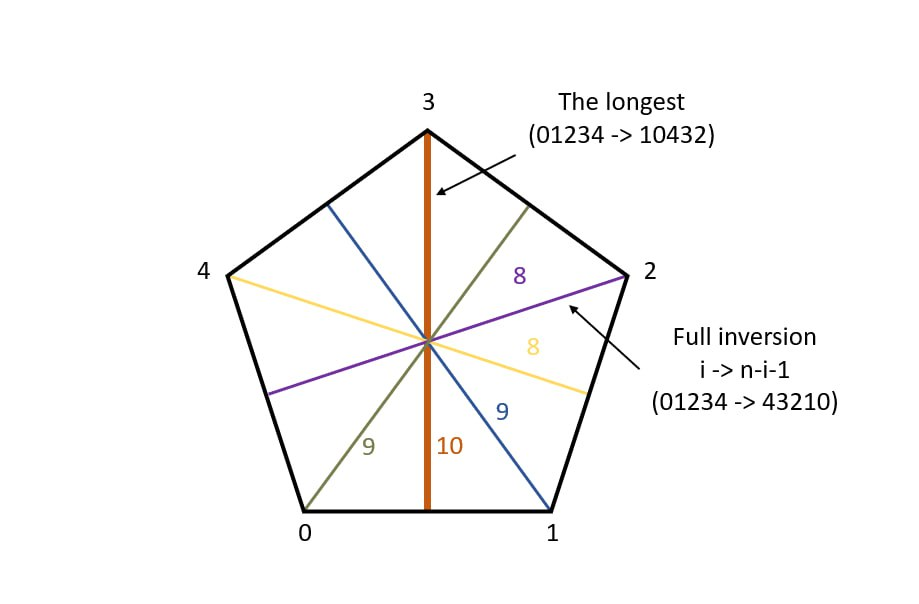
\includegraphics[width=1.0\linewidth]{figs/LongEl.jpg}
   \caption{Permutations arising from dihedral symmetries - are provebly long elements. The longest is conjecturally one of them. Surprisingly it is not the full inversion.}\label{fig:LongEl}
\end{figure}

We created efficient implementation of the brute force breadth first search algorithm \href{https://www.kaggle.com/code/ivankolt/lrx-4bit-uint64}{notebook} using bit operations over int64 and were able to traverse all the permutations for $n \le 14$, outperforming OEIS data by one step. From that computation we observed that the longest element is unique and have a specific form. It can be described as a symmetry of a regular polygon. Orthogonal to 0-1 edge. Or explicitly as product of transpositions $(0,1)(n-1,2)(n-2,3)(n-3,3)...$. We conjecture that this element is unique longest element and it has length $n(n-1)/2$. 
Surprisingly that element, but not the full inversion $i\to n-i-1$ is the longest. 

As we will prove below actually all the permutations which correspond to  symmetries of a regular polygon are also long elements.  


\begin{proposition}
    The element $(0,1)(n-1,2)(n-2,3)(n-3,3)...$ (conjecturally the longest)
    has the following explicit decomposition into product of LRX generators.
\begin{equation}
\label{eq:long}
\prod_{i=1}^{[ (n-1)/2]} ( X L^{(-1)^{(i-1)}} )^i 
\prod_{i=([ n/2]-1)}^{1} (L^{(-1)^{i+[(n-1)/2] - [n/2] }} X )^i R^{[n/2]}
\end{equation}    
\end{proposition}
The proof will be given elsewhere. The decompositions of that pattern were first found computationally \href{https://www.kaggle.com/code/luxoove/lrx-optimal-algorithm-two-ways-bubble-sort}{notebook}.

%\subsection{The long elements,  and the formula for the longest one}


\subsection{Lower bound on the diameter}
Below we will give a lower bound on the diameter by the combinatorial argument, the idea is that cyclic shifts do not change the cyclic order on any triple of number, and so for each triple with broken order  we need $X$  in the  decomposition. The symmetries of regular polygon described above are precisely  permutations which change the cyclic order as much as possible. More careful arguments are below. The code to generate these long elements: \href{https://www.kaggle.com/code/alexandervc/lrx-long-elements-f-petrov-oeisa186752}{notebook}. 

\begin{proposition}
    Diameter of LRX graph is larger or equal $n(n-1)/2-n/2$ 
\end{proposition}

At first, we reformulate the setup as follows.

The numbers $1,\ldots,n$  are written in the vertices of a regular $n$-gon $A_1A_2\ldots A_n$, each number being written once. At each move, one can either rotate the arrangement by $2\pi/n$  counterclockwise or clockwise, or switch the numbers at $A_1$ and $A_2$.

For two arrangements $\pi_1,\pi_2$ denote by $d(\pi_1,\pi_2)$ the minimal number of moves which suffice to get $\pi_2$ from $\pi_1$.

Claim. If $\pi_2$ is obtained from $\pi_1$ by an axial symmetry, then $d(\pi_1,\pi_2)\geqslant n^2/2-n-1$.

Proof. Assume that $\pi_2$ is obtained from $\pi_1$ by several moves. Call two numbers $a, b\in \{1,\ldots,n\}$ friends, if they were switched odd number of times. Since for every three numbers $a, b, c$ the orientation of a triangle formed by these numbers changed, there is odd number of pairs of friends between $a, b, c$. Let $A$ denote the set of all non-friends of element 1, $B$ the complement  of $A$, i. e. $B$ consists of 1 and its friends. Our condition yields that all elements of $A$ are mutual friends, and so are all elements of $B$, but there is no friendship between $A$ and $B$. Thus, the total number of pairs of friends is $n(n-1)/2-|A|\cdot |B|\geqslant n(n-1)/2-n^2/4$. Thus there were at least as many switches. Between every two switches there was a rotation (otherwise we do something useless). Totally, the number of operations is not less than $n(n-1)-n^2/2-1=n^2/2-n-1$.

\subsection{Upper bound on the diameter and the algorithms }
We develop two algorithm which can decompose any permutation in the product of LRX generators. Its complexity is  $n(n-1)/2+3n$, thus giving such an upper bound for the diameter.  The code and tests for the first one can be found in \href{https://www.kaggle.com/code/mixnota/article-project}{notebook}.

Its brief description is the following:

The algorithm decomposes a permutation into the product of cycles. After that, it works with each cycle \( (a_1, a_2, \dots, a_n) \) in the following way:

1) We compute the permutation corresponding to the cycle.

2) We initialize the special variable \( x \).

3) The element \( a_1 \) is placed in the \( a_n \)-th position, and we perform a sequence of elementary transpositions to move \( a_1 \) from the \( a_n \)-th position to the \( a_1 \)-th position. During each elementary transposition, we either increase or decrease \( x \) by 1. The sign of the change depends on the direction of the elementary transposition. Essentially, \( x \) represents the current position of the transposition, but if our transposition is \( (1, N) \), the change in \( x \) is also \( \pm1 \), even though the position changes from 1 to \( N \) or from \( N \) to 1.

4) Next, we attempt to restore the position of \( a_2 \) and compute the sequence of elementary transpositions that move \( a_2 \) to the \( a_2 \)-th position. We apply the same operations to \( x \), and so on.

5) We repeat these actions for every element of the cycle.

6) In certain situations, the elementary transposition should be replaced by \( L \) or \( R \) (depending on the direction in which we are moving the current element). This replacement should occur if and only if the variable \( x \) satisfies the condition:

\[
x - c = \pm (N - 1)
\]


Its complexity estimation.
First, when decomposing a cycle into transpositions, we do not shift anything by more than 1, except for elements that have already been affected by the cycle.
Second, when moving an element from position \( i \) (or \( i \pm 1 \)) to position \( \sigma(i) \), we perform a sequence of at most \( \text{dist}(i, \sigma(i)) + 1 \) transpositions.
Third, the transition from \( i \to \sigma(i) \) to \( \sigma(i) \to \sigma(\sigma(i)) \) takes at most one rotation.
Thus, we perform at most  
\[
\sum 2(\text{dist}(i, \sigma(i)) + 1) + (\text{number of elements in the cycle})
\]
operations. The transitions between cycles and returning back will take at most \( n \) rotations.
Therefore, the entire decomposition takes no more than  
\[
2n + \sum 2(\text{dist}(i, \sigma(i)))
\]
operations.

Finally, after minimization,
\[
\sum \text{dist}(i, \sigma(i)) \leq \frac{n^2}{4}
\]
which gives a total of  
\[
2n + \frac{n^2}{2} + \frac{n}{2}
\]
operations.




The second is implemented in \href{https://www.kaggle.com/code/luxoove/top1-lrx-inversions-based-algorithm}{notebook} currently it is our top performing algorithm from the practical tests, we expect its worst case length output is $n(n-1)/2+n/2$, however it is not yet proved.


\subsection{Conjectures: Gumbel for growth, spectrum uniformity, random walks mixing, etc. }

Based on explicit computations for the growth for $n \le 14$ and its analysis (notebooks \href{https://www.kaggle.com/code/ogurtsov/gumbel}{1} \href{https://www.kaggle.com/code/ogurtsov/gumbel-for-binary-puzzle}{2} ) we come to the following conjecture, which can be thought as an analogue of the central limit theorems. 

{\bf The growth - Gumbel.} The growth distribution of the LRX graph follows the Gumbel distribution for large $n$.

\begin{figure}[h!]
   \centering
   \includegraphics[width=1.0\linewidth]{figs/LRX_spec.png}
   \caption{Spectrum distribution of the LRX graphs. }\label{fig:LRX-spec}
\end{figure}

The analysis of the spectrum of LRX graphs is perfomed in \href{https://www.kaggle.com/code/nikolenkosergei/spectrum-analysis}{notebook}. From the figure above it is natural to expect that spectrum tends to uniform distribution.

We have computed all possible shortest paths from the conjecturally longest element to the identity by methods of the dynamical programming (\href{}{notebook} ). And after that analyzed averages trajectories (\href{https://www.kaggle.com/code/antoninadolgorukova/lrx-sorting-networks}{notebook}) - which are analogs of sorting networks \cite{angel2007random}. The figure below represents the results. It seems the pattern is different from the "sine curves" discovered in \cite{angel2007random}. 

\begin{figure}[h!]
   \centering
   \includegraphics[width=1.0\linewidth]{figs/LRX_sorting.jpg}
   \caption{Analogs of "sorting networks" for LRX. Trajectories of individual elements under average of all possible shortest trajectories between longest node and identity. }\label{fig:LRX-sort}
\end{figure}

We also numerically checked for even  $n \le 9$ (\href{https://www.kaggle.com/code/fedmug/lrx-shifts-starting-with-x}{notebook}) the following conjecture. It   would imply precise diameter lower bound $n(n-1)/2$. 

{\bf Conjecture.} If the shortest  decomposition of an element starts from $X$, then its multiplications by $L^k$ $k<n/2$  have all different lengths.  

Such a conjecture imply that half of the symmetries of the regular polygon have different lengths, but since their lengths greater than $n(n-1)/2-n/2$ one of the would have length $n(n-1)/2$ which is desired diameter. 

\section{Code availability}

The code is available at the Kaggle platform, where it can be easily launched:
\href{https://www.kaggle.com/competitions/lrx-oeis-a-186783-brainstorm-math-conjecture/code}{LRX OEIS-A186783 brainstorm math conjecture}

The link above is one  the three  created public Kaggle challenges to stimulate the research and interplay between artificial intelligence and mathematical communities, the other two:
\href{https://www.kaggle.com/competitions/lrx-binary-in-search-of-gods-number}{LRX discover math and God's algorithm}, \href{https://www.kaggle.com/competitions/lrx-discover-math-gods-algorithm}{LRX-binary: in search of God's number}.


\section{Acknowledgments}
A.C. is deeply grateful to M. Douglas for his interest in this work, engaging discussions, and invitation to present preliminary results at the Harvard CMSA program on "Mathematics and Machine Learning" in Fall 2024, to M. Gromov, S. Nechaev, and V. Rubtsov for their invitation to make a talk at "Representations, Probability, and Beyond: A Journey into Anatoly Vershik World" at IHES, as well as for stimulating discussions. A.C. is grateful to J. Mitchel for involving  into the Kaggle Santa 2023 challenge, from which this project originated and to M.Kontsevich, Y.Soibelman,  S.Gukov, A. Hayat, T. Smirnova-Nagnibeda,  D.Osipov, V. Kleptsyn, G.Olshanskii, A.Ershler, J. Ellenberg, G. Williamson, A. Sutherland,  Y. Fregier, P.A. Melies, I. Vlassopoulos, F.Khafizov, A.Zinovyev,  H.Isambert for the discussions, interest and comments. 

We are deeply grateful to the many colleagues who have contributed to the CayleyPy project at various stages of its development, including: N.Bukhal, J.Naghiev, A.Lenin, E.Uryvanov,  A. Abramov, M.Urakov, A.Kuchin,  B.Bulatov,  F.Faizullin, A.Aparnev, O.Nikitina, A.Titarenko, U.Kniaziuk, D.Naumov, A.Krasnyi, S.Botman,
R.Vinogradov, I.Gaiur, I.Kiselev,  % added
% D.Gorodkov, A.Rozanov,V.Nelin,  A. Ogurtsov, A. Trepetsky, A. Dolgorukova, S. Lytkin, S. Ermilov, L. Grunvald, A. Eliseev, G. Annikov, M. Evseev, F. Petrov, N. Narynbaev, S. Nikolenko, S. Krymskii, R. Turtayev, S. Kovalev, N. Rokotyan, G. Verbyi, L. Shishina, A.Korolkova, D.Mamaeva,  S.Fironov, A.Lukyanenko,
K.Yakovlev, V.Shitov, E.Durymanov, A.Kostin, R.Magdiev, M.Krinitskiy, P.Snopov. 

%The classical Rubik's cube is a 3D puzzle with about $4.3\times 10^{19}$ possible states. Although this number is too large to use classical dynamic programming methods, the much smaller \href{https://en.wikipedia.org/wiki/Pocket_Cube}{Pocket Cube} with its $3.67$\footnote{$3674160$, to be precise (see, e.g., \cite[p.31]{singmaster1981notes}} million states still provides a rich problem space for exploration. This balance of reduced complexity and meaningful scale makes the Pocket Cube an excellent testing ground for evaluating and comparing tabular RL algorithms, offering insights into their ability to find the shortest path to the target state.

%\subsection{Cayley graphs on the Pocket Cube} \label{cayley-graphs}

%We represent each \textit{state} $s$ of the Pocket Cube by a permutation from $S_{24}$. The \textit{solved} (\textit{target}) state $s_0$ is the identity permutation. A \textit{move} (or \textit{action}) $a\in \mathcal A$ is a specific rotation of the cube which can also be written as such a permutation. Taking a move $a$ in state $s$ we arrive at a new state $s'=a\circ s$. All possible moves 

%$$\mathcal A = \{f_0, f_0^{-1}, f_1, f_1^{-1}, r_0, r_0^{-1}, r_1, r_1^{-1}, d_0, d_0^{-1}, d_1, d_1^{-1}\}, $$

%\noindent
%are 90 degree rotations of the front, right, and down faces. For example, the rotations of the nearest front face are given by

%$$
%f_0 = (2\ 19\ 21\ 8) (3\ 17\ 20\ 10) (4\ 6\ 7\ 5), \quad
%f_0^{-1} = (2\ 8\ 21\ 19)(3\ 10\ 20\ 17)(4\ 5\ 7\ 6).
%$$

%\begin{figure}[h!]
%    \centering
%    \includegraphics[width=1.0\linewidth]{figs/f0.png}
%    \caption{Rotating the front face $90$ degrees clockwise from the solved state (visualization is based on \href{https://www.kaggle.com/code/marksix/visualize-allowed-moves}{this Kaggle notebook})}\label{fig:f0-move}
%\end{figure}

%Let $G = G(a_1, \ldots, a_k)$, $a_1\ldots, a_k \in \mathcal A$, be the Cayley graph which corresponds to a subgroup of $S_{24}$ generated by 

%$$
%    \bigcup\limits_{i=1}^k \{a_i, a_i^{-1}\}.
%$$

%Solving the puzzle means finding a path (preferably, the shortest one)  from any state $s \in G$ to the target in this graph. Running the BFS algorithm from $s_0$ we split our graph $G$ into several disjoint layers $G_k$ such that the length of the shortest path from any vertex $s \in G_k$ to $s_0$ is $k$. The number of layers equals the diameter of $G$, also known as \textit{God's number} (in QTM). The God's number for the Pocket Cube is known to be $14$ (see \href{http://www.math.rwth-aachen.de/~Martin.Schoenert/Cube-Lovers/Jerry_Bryan__God's_Algorithm_for_the_2x2x2_Pocket_Cube.html}{this ancient link}), and it matches the results of BFS summarized in Table~\ref{tab:layer_sizes} (see columns for $G(f_0, r_0, d_0)$ and $G(\mathcal A)$). Note that for other sets of generators the diameter of $G$ could be different.

%\begin{table}[h!]
%\centering
%\begin{tabular}{lccccc}
%\toprule
%\textbf{Graph}       & $G(f_0, r_0)$  & $G(f_0, r_0, d_0)$ & $G(f_0, f_1, r_0, r_1)$   & $G(f_0, f_1, r_0, d_0)$  & $G(\mathcal A)$\\
%\midrule
%Layer 0    &  1 & 1 & 1 & 1 & 1 \\
%Layer 1    &  4 & 6 & 8 & 8 & 12 \\
% Layer 2    &  10 & 27 & 44 & 48 & 114 \\
% Layer 3    &  24 & 120 & 232 & 272 & 924 \\
% Layer 4    &  58 & 534 & 1226 & 1525 & 6539 \\
% Layer 5    &  130 & 2256 & 5996 & 8214 & 39528 \\
% Layer 6    &  271 & 8969 & 28016 & 41986 & 199926 \\
% Layer 7    &  526 & 33058 & 123124 & 202044 & 806136 \\
% Layer 8    &  980 & 114149 & 511449 & 910137 & 2761740 \\
% Layer 9    &  1750 & 360508 & 1956336 & 3737518 & 8656152 \\
% Layer 10    &  2731 & 930588 & 6855860 & 13086347 & 22334112 \\
% Layer 11    &  3905 & 1350852 & 19813152 & 30652249 & 32420448 \\
% Layer 12    &  5229 & 782536 & 33501130 & 29933084 & 18780864 \\
% Layer 13    &  5848 & 90280 & 22185904 & 9489615 & 2166720 \\
% Layer 14    &  4792 & 276 & 3192194 & 116792 & 6624 \\
% Layer 15    &  2375 & -- & 5168 & -- & -- \\
% Layer 16    &  508 & -- & -- & -- & -- \\
% Layer 17    &  18 & -- & -- & -- & -- \\
% \midrule
% \textbf{Total} &  \textbf{29160} & \textbf{3674160} & \textbf{88179840} & \textbf{88179840} & \textbf{88179840} \\
% \bottomrule
% \end{tabular}
% \smallskip
% \caption{Sizes of layers of Cayley graphs for different generators}
% \label{tab:layer_sizes}
% \end{table}

%\subsection{Dynamic programming} \label{DP}

%In this subsection, we apply basic reinforcement learning techniques, such as value and policy iteration, to solve the Pocket Cube puzzle. For each state $s \in \mathcal S = G(f_0, r_0, d_0)$ the reference solution 

%$$  d(s) = \rho(s, s_0) =  \min\limits_{\mathrm{path}(s_0, s)} |\mathrm{path}(s_0, s)|
%$$

%\noindent
%has already been found by BFS in the previous section (see also column 2 of the Table~\ref{tab:layer_sizes}), and here we will use it as a benchmark for RL algorithms.
 
%Note that $d(s)$ satisfies the \textit{Bellman equation}

%\begin{equation}
%\label{eq:min_bellman}
%d(s) = 1 + \min\limits_a d(a\circ s), \quad s \ne s_0, \quad d(s_0) = 0.
%\end{equation}


%To solve this equation we use dynamic programming (DP) algorithm.

% \begin{algorithm}[H]
% \caption{Dynamic programming}
% \begin{algorithmic}[1]
% \STATE \textbf{Hyperparameters:} $\epsilon > 0$ (tolerance), $\alpha \in (0, 1]$ (learning rate), $N$ (maximum iterations)
% \STATE Initialize $d_0(s)$ for all states $s \in \mathcal S$ (e.g., by zeros)
% \FOR{$i = 0$ to $N$}
%     \STATE $d_{i+1}(s_0) \leftarrow 0$
%     \FOR{each state $s \ne s_0$}
%         \STATE 
%         $d_{i+1}(s) \leftarrow  \alpha(1 + \min\limits_a d_i(a\circ s)) + (1-\alpha)d_i(s)$
%     \ENDFOR
%     \STATE
%     $c_i \leftarrow \mathrm{corr}(\boldsymbol d_i, \boldsymbol d)$
%     \IF {$\Vert \boldsymbol d_i - \boldsymbol d\Vert  < \epsilon$}
%         \STATE \textbf{break}
%     \ENDIF
% \ENDFOR
% \STATE \textbf{Output:} Number of iterations $i$, vector of correlations $\boldsymbol c$ 
% \end{algorithmic}
% \end{algorithm}

% Since we know the true distances $d(s)$ for $2\times 2 \times 2$ cube, we can easily check whether the process has converged or not: when $\|d_n(s) - d(s)\| < \varepsilon$, we are finished.

% We try different initializations $d_0(s)$:

% \begin{itemize}
% \item 
% zero initialization $d_0(s) = 0$ for all $s$
% \item 
% initialize each layer by a specific value (e.g., first $k$ layers by true distances, last $14 - k$ layers by zeros, $1 \leqslant k < 14$)
% \item
% Manhattan distance to the target: 
% $d_0(s) = \sum\limits_{k=0}^{23} \vert s_k - k \vert$
% \item 
% Hamming distance to the target:
% $d_0(s) = \vert \{k\colon s_k \ne k\}\vert$

% \item 
% Random integers form $0$ to $14$ or random values from $\mathcal N(0, \sigma^2)$
% \end{itemize}

%For each $\alpha = \frac j{10}$, $1\leqslant j \leqslant 10$, run the DP algorithm with different initialization strategies until convergence. From the results presented in Fig.~\ref{fig:iterations} we conclude that the number of iterations is a decreasing function of $\alpha$, and for $\alpha=1$ the algorithm converges in $14$ iterations (diameter of the graph) in all cases except one, when starting values are drawn from $\mathcal N(0, 5)$. On the other hand, the type of initialization of $d_0(s)$ does not have a substantial impact on the rate of convergence.

%\begin{figure}[h!]
%    \centering
%    \includegraphics[width=1.0\linewidth]{figs/iterations.png}
%    \caption{Number of iterations required for convergence of the DP algorithm with %$\epsilon = 10^{-3}$}\label{fig:iterations}
%\end{figure}

%Another measure of convergence is the correlation between the current approximation $d_i(s)$ and the true distances $d(s)$. Fig.~\ref{fig:pearson} shows the graphs of such Pearson correlations for $\alpha = 1$ and $\alpha=0.8$. Interestingly, they reveal non-monotonic nature of $\mathrm{corr}(\boldsymbol d_i, \boldsymbol d)$ for some types of initializations $d_0(s)$ (e.g., by true distances of first $13$ layers or random walk init). The Gaussian initialization demonstrates the worst behavior: the correlations can oscillate around $0$ for a long time before finally converge to $1$. In our experiments, this effect disappears after clipping negative values of $d_0(s)$
%  to zero.
% \begin{figure}[h]
%     \centering
%     \includegraphics[width=1.0\linewidth]{figs/pearson.png}
%     \caption{Pearson correlation between $d_i(s)$ and $d(s)$ on each iteration of the DP algorithm, $\epsilon = 10^{-3}$}\label{fig:pearson}
% \end{figure}


% \subsection{Value iteration}\label{VI}

% The problem of finding the shortest path in the Cayley graph $G$ can be reformulated in terms of reinforcement learning. Suppose we are training an agent to solve Rubik's cube. After taking action $a$ in state $s$ the agent goes to state $s'$, and receives reward $r(s, a) = -1$.
% The goal is to maximize the total cumulative reward. Clearly, this is the same as finding the shortest route from $s$ to $s_0$.

% The \textit{value function} $v_*(s)$ (\cite[p.62]{Sutton1998}) shows how good the state $s$ is. This function satisfies the \textit{Bellman optimality equation}

% $$
%     v_*(s) = \max\limits_a \big\{r(s, a) + \gamma \mathbb E_{s'} v_*(s')\big\}
% $$

% \noindent
% where $\gamma \in(0,1]$ is \textit{discount factor}. Our environment is deterministic, hence, $\mathbb E_{s'} v_*(s') = v_*(a\circ s)$ and

% \begin{equation}
%     \label{eq:v-star-bellman}
%     v_*(s) =
%         -1+ \gamma\max\limits_a \big\{v_*(a\circ s)\big\}
% \end{equation}

% \noindent
% (assume $v_*(s_0) = 0$). Now observe that~\ref{eq:min_bellman} turns into~\ref{eq:v-star-bellman} if $\gamma = 1$ and $d(s) = -v_*(s)$.

% \bigskip

% Describe dyn-prog-Q-alg.

% Discuss experiments:

% 1) Convergence less than diameter of positive initiliazation

% 2) If negative more steps than diameter;

% 3) Shows effects of different initialization



% \section{Deep Reinforcement learning on huge graphs}

% \section{Methods}

% \subsection{Bellman equation on graphs}
% \label{SecBellman}

% {\bf Question: } Find analogue for diffusion distance. Standard Bellman - should be "tropical limit".




% \subsection{DQN}
% \label{SecDQN}


% \subsection{PPO}
% \label{SecPPO}

% \subsection{Cayley graphs}
% \label{SecCayley}

% \subsubsection{Cayley Graph generated by neighbor transpositions - 1-skeleton of the Permutohedron}

% \subsubsection{Cayley Graph generated by all transpositions}

% \subsubsection{Cayley Graph generated by (1,2) and long cycle}



% \subsection{Limits of GAP. ("Overcome the GAP")}
% \label{SecGAP}

% We explore the performance of GAP on several generator sets of $S_n$. 
% In particular we analyze the lengths of the obtained decompositions, how big $n$ GAP can support and timing. 


% \subsubsection{GAP on Cayley Graph generated by neighbour transpositions - 1-skeleton of the Permutohedron}

% \subsubsection{GAP on Cayley Graph generated by all transpositions}


% \subsubsection{GAP on Cayley Graph generated by (1,2) and long cycle}

% \begin{figure}[b]
%     \centering
%     \includegraphics[width=0.7\linewidth]{figs/length.png}
%     \caption{The average length of an element in a group $S_n$, as a function of the length of the permutations n,, on both a standard and logarithmic scale.}\label{fig:enter-label}
% \end{figure}

% This section provides an analysis of the GAP's capabilities when defining a group $S_n$ using two cycles: $(1\ 2)$ and $(1\ 2\ ...\ n)$.The experiments were conducted using a CPU with 30 GB of RAM and a TPU with 330 GB of RAM.GAP algorithms have exceeded the memory limit for $n = 33$ on TPU and $n = 31$ on CPU.
% From Figure 1 it is evident that the average element length grows faster than $O(e^n)$.


%\providecommand{\href}[2]{#2}
\printbibliography
% \address{
% Alexander Chervov - Institut Curie,\\
% 26 rue d'Ulm, 75248 Paris, France\\
% \email{al.chervov@gmail.com}\\
% }


\end{document}
